\documentclass[11pt]{article}

\usepackage[margin=0.85in]{geometry}
\usepackage[T1]{fontenc}
\usepackage[utf8]{inputenc}
\usepackage{lmodern}
\usepackage{amsmath,amssymb,mathtools}
\usepackage{booktabs,longtable,array}
\usepackage{graphicx}
\usepackage{pdflscape}
\usepackage{microtype}
\usepackage{caption}
\usepackage{hyperref}

\hypersetup{
  colorlinks=true,
  allcolors=black,
  linkcolor=black,
  urlcolor=black,
  citecolor=black,
  pdftitle={Ceros exactos de Lee--Yang, susceptibilidad autodual y escalamiento de la brecha de Lee--Yang en modelos cilíndricos SOS multicapa}
}
\graphicspath{{./}}
\setlength{\emergencystretch}{2em}
\newcommand{\Z}{\mathbb{Z}}
\newcommand{\Ocal}{\mathcal{O}}
\newcommand{\tablevalue}[1]{\texttt{#1}}
\newcommand{\tableheading}[2]{\multicolumn{1}{>{\centering\arraybackslash}p{#1}}{#2}}

\title{Ceros exactos de Lee--Yang, susceptibilidad autodual y escalamiento de la brecha de Lee--Yang en modelos cilíndricos SOS multicapa}
\author{Wendel León Alvarado}
\date{12 de noviembre de 2026}

\begin{document}
\maketitle

\begin{abstract}
Relacionamos los posets corona cilíndricos multicapa, las configuraciones de altura monótonas tipo solid-on-solid (SOS) y las funciones de partición finitas de Lee--Yang. El numerador de Ehrhart $H_{k,n}(t)$ del politopo de orden de $C_{k,n}$ es el polinomio generador de descensos de sus extensiones lineales; sus coeficientes son conteos microcanónicos de excitaciones y $t$ es una fugacidad gran-canónica. Certificados exactos y contracciones Tensor-CRT proporcionan 23 polinomios palindrómicos para perímetros $3\le n\le7$, cuyos ceros fueron aislados en el eje real negativo y refinados a 50 dígitos decimales. Las raíces recíprocas dan una representación factorizada de cuasipartículas para la energía libre, la densidad de excitaciones y la susceptibilidad. La palindromicidad prueba la dualidad $\chi(1/t)=\chi(t)$; certificados exactos adicionales de positividad muestran que $t=1$ es el máximo global único en cada una de las 23 instancias finitas. Para $n=3$, una recurrencia exacta de dos modos prueba que la energía libre termodinámica es analítica para toda fugacidad positiva. Presentamos las tasas de contracción de la brecha para perímetros finitos y comparamos las distribuciones empíricas de $H_{8,3}$ y $H_{8,4}$ con sus densidades de fase BKW. La curva BKW para $n=4$ depende de extender su recurrencia observada de orden tres a todas las longitudes.
\end{abstract}

\noindent\textbf{Palabras clave:} ceros de Lee--Yang; politopos de orden; P-particiones; modelos solid-on-solid; polinomios recíprocos; susceptibilidad; teoría de Beraha--Kahane--Weiss.

\section{Introducción y correspondencia estadístico-mecánica exacta}

Sea $C_{k,n}$ el poset corona cilíndrico con vértices $x_{j,i}$, donde $1\le j\le k$ es la capa e $i\in\Z/n\Z$ es la coordenada cíclica. Sus relaciones de cubierta son
\[
  x_{j,i}\prec x_{j+1,i},\qquad x_{j,i}\prec x_{j+1,i+1}
  \quad (1\le j<k).
\]
Denotamos por $d=kn$ el número de vértices. El politopo de orden es
\[
  \Ocal(C_{k,n})=\{y\in[0,1]^d:y_u\le y_v\text{ cuando }u\preceq v\}.
\]
Su conteo de Ehrhart y su numerador se definen mediante
\begin{equation}
  L_{k,n}(m)=|m\Ocal(C_{k,n})\cap\Z^d|,
  \qquad
  \sum_{m\ge0}L_{k,n}(m)z^m=\frac{H_{k,n}(z)}{(1-z)^{d+1}}.
  \label{eq:es-ehrhart}
\end{equation}
Así, $L_{k,n}(m)$ cuenta exactamente las configuraciones de alturas SOS enteras
\[
  h_{j,i}\in\{0,1,\ldots,m\},\qquad
  h_{j,i}\le h_{j+1,i},\quad h_{j,i}\le h_{j+1,i+1},
\]
en el grafo cilíndrico dirigido de cubiertas. Es un modelo RSOS monótono con cota dura de altura: $m$ es el corte microcanónico y $L_{k,n}(m)$ es el conteo exacto de configuraciones. Las desigualdades escritas contienen todas las interacciones; no se impone una restricción adicional de vecinos más próximos a través de la circunferencia.

Etiquetamos naturalmente los vértices mediante $n(j-1)+i+1$. La descomposición en P-particiones de las aplicaciones que preservan el orden da
\begin{equation}
  H_{k,n}(t)=\sum_{\pi\in\mathcal{L}(C_{k,n})}t^{\operatorname{des}(\pi)}
  =\sum_{q=0}^{D}h_q^*t^q,
  \qquad D=d-k=k(n-1),
  \label{eq:es-partition}
\end{equation}
donde $\mathcal{L}(C_{k,n})$ es el conjunto de extensiones lineales y los descensos se miden en el etiquetado natural. Por tanto, $h_q^*$ es el número microcanónico de estados de extensión con $q$ excitaciones de descenso, y
\[
  Z_{k,n}(t):=H_{k,n}(t)=\sum_{q=0}^{D}h_q^*t^q
\]
es su función de partición gran-canónica finita. Sus ceros complejos son ceros de Lee--Yang en la variable de fugacidad $t$ para este sistema finito \cite{LeeYang1952}. El conteo con cota de altura $L_{k,n}(m)$ y la función de partición de excitaciones $H_{k,n}(t)$ son ensambles distintos, relacionados por la función generatriz de Ehrhart \eqref{eq:es-ehrhart}.

Los posets corona son graduados y sus polinomios $h^*$ son Gorenstein y palindrómicos:
\begin{equation}
  h_q^*=h_{D-q}^*,\qquad H_{k,n}(t)=t^D H_{k,n}(1/t).
  \label{eq:es-reciprocal}
\end{equation}
Usamos los certificados JSON disponibles para $n=3,4,5$ y $k\le8$. Las contracciones Tensor-CRT reconstruyen además $H_{3,6}$, $H_{4,6}$ y $H_{3,7}$. Para comparar con BKW en $n=4$ también calculamos $H_{8,4}$, ya que no existe un archivo de certificado para $C_{8,4}$. El estudio reúne 23 polinomios. Aislamos las raíces con intervalos racionales exactos de la reducción recíproca y las refinamos con aritmética mpmath de 75 dígitos; se reportan 50 cifras significativas.

\section{Ausencia de transición de fase a fugacidad positiva para cilindros angostos}

Para perímetro tres, una transferencia exacta prueba para todo $k\ge2$ la recurrencia
\begin{equation}
  H_{k,3}(t)=P_3(t)H_{k-1,3}(t)+Q_3(t)H_{k-2,3}(t),
  \quad P_3(t)=t^2+6t+1,\quad Q_3(t)=t(t-1)^2,
  \label{eq:es-n3-recurrence}
\end{equation}
con $H_{0,3}=1$ y $H_{1,3}=t^2+4t+1$. Sus raíces características son
\begin{equation}
  \lambda_\pm(t)=\frac{P_3(t)\pm\sqrt{P_3(t)^2+4Q_3(t)}}{2}.
  \label{eq:es-n3-eigenvalues}
\end{equation}
Para todo $t>0$, $P_3(t)>0$, $Q_3(t)\ge0$ y el discriminante es estrictamente positivo. Por ello, $\lambda_+(t)>0$ es simple y domina estrictamente a $|\lambda_-(t)|$. El coeficiente de $\lambda_+^k$ en la solución es
\[
  A_+(t)=\frac{H_{1,3}(t)-\lambda_-(t)}{\lambda_+(t)-\lambda_-(t)}>0.
\]
Se sigue, localmente de manera uniforme para $t>0$, que
\begin{equation}
  f_{\infty,3}(t):=\lim_{k\to\infty}\frac{1}{3k}\log H_{k,3}(t)
  =\frac13\log\lambda_+(t).
  \label{eq:es-free-energy-limit}
\end{equation}
El lado derecho es real-analítico para toda fugacidad positiva. Por tanto, el modelo de longitud infinita con perímetro fijo tres no tiene singularidad termodinámica sobre el eje real positivo. Esta afirmación se refiere al límite en longitud de capas con perímetro tres fijo; no descarta transiciones en límites donde también crece el perímetro.

El mismo análisis espectral confina todos los ceros finitos para $n=3$ al intervalo
\begin{equation}
  I_3=(-7-4\sqrt3,-7+4\sqrt3)\subset(-\infty,0).
  \label{eq:es-i3}
\end{equation}
En particular, el eje de fugacidad positiva queda separado de los ceros de Lee--Yang. La recurrencia de $n=3$, el confinamiento y la simplicidad de raíces son exactos para todo $k\ge2$; la tabla numérica es una muestra finita del teorema.

\section{Cuasipartículas de Pitman y susceptibilidad autodual}

Para las instancias estudiadas, las raíces $r_1,\ldots,r_D$ son simples y estrictamente negativas, y $H_{k,n}(0)=1$. Por tanto,
\begin{equation}
  H_{k,n}(t)=\prod_{j=1}^{D}\left(1-\frac{t}{r_j}\right),
  \qquad p_j(t)=\frac{t}{t-r_j}.
  \label{eq:es-pitman-factorization}
\end{equation}
Cada factor es la función de partición de un modo de dos estados con ocupación $p_j(t)$. La representación independiente de cuasipartículas de Pitman da
\begin{align}
  f_{k,n}(t)&=\frac{1}{kn}\log H_{k,n}(t),\\
  u_{k,n}(t)&=\frac{1}{kn}\sum_{j=1}^{D}p_j(t),\\
  \chi_{k,n}(t)&=\frac{1}{kn}\sum_{j=1}^{D}p_j(t)(1-p_j(t))
  =\frac{1}{kn}\sum_{j=1}^{D}\frac{-t r_j}{(t-r_j)^2}.
  \label{eq:es-thermodynamics}
\end{align}
Aquí $u$ es la densidad de excitaciones y $\chi$ su respuesta a la fugacidad (el análogo del calor específico en esta convención adimensional).

La reciprocidad \eqref{eq:es-reciprocal} implica una dualidad directa. Sea $U(t)=tH'_{k,n}(t)/H_{k,n}(t)=kn\,u_{k,n}(t)$. Al derivar la identidad recíproca,
\[
  U(1/t)=D-U(t).
\]
Como $\chi(t)=tU'(t)/(kn)$, una segunda derivación prueba
\begin{equation}
  \chi_{k,n}(1/t)=\chi_{k,n}(t),
  \qquad u_{k,n}(1/t)=\frac{n-1}{n}-u_{k,n}(t).
  \label{eq:es-duality}
\end{equation}
La susceptibilidad es estacionaria en la fugacidad autodual $t=1$. La palindromicidad por sí sola no demuestra que ese punto sea un máximo. Para los 23 polinomios exactos de este estudio establecemos el resultado finito más fuerte mediante un certificado adicional de positividad.

Definamos
\[
  N_{k,n}(t)=tH_{k,n}H'_{k,n}+t^2H_{k,n}H''_{k,n}-t^2(H'_{k,n})^2.
\]
Entonces $\chi_{k,n}(t)=N_{k,n}(t)/(knH_{k,n}(t)^2)$. La aritmética entera exacta da, para cada uno de los 23 polinomios,
\begin{equation}
  N_{k,n}(1)H_{k,n}(t)^2-N_{k,n}(t)H_{k,n}(1)^2
  =(t-1)^2 C_{k,n}(t),
  \qquad C_{k,n}(t)\in\Z_{\ge0}[t]\setminus\{0\}.
  \label{eq:es-peak-certificate}
\end{equation}
El generador de figuras verifica directamente esta condición para cada vector de coeficientes. Como $H_{k,n}(t)>0$ para $t>0$, la ecuación \eqref{eq:es-peak-certificate} prueba que $\chi_{k,n}(1)>\chi_{k,n}(t)$ para todo $t>0$, $t\ne1$, en las 23 instancias. Así, el máximo global único de susceptibilidad es exactamente
\begin{equation}
  t^*(k,n)=1.
  \label{eq:es-peak}
\end{equation}
Es un resultado certificado para los polinomios enumerados; no afirmamos que la positividad se haya demostrado para todo $k,n$.

\begin{figure}[htbp]
  \centering
  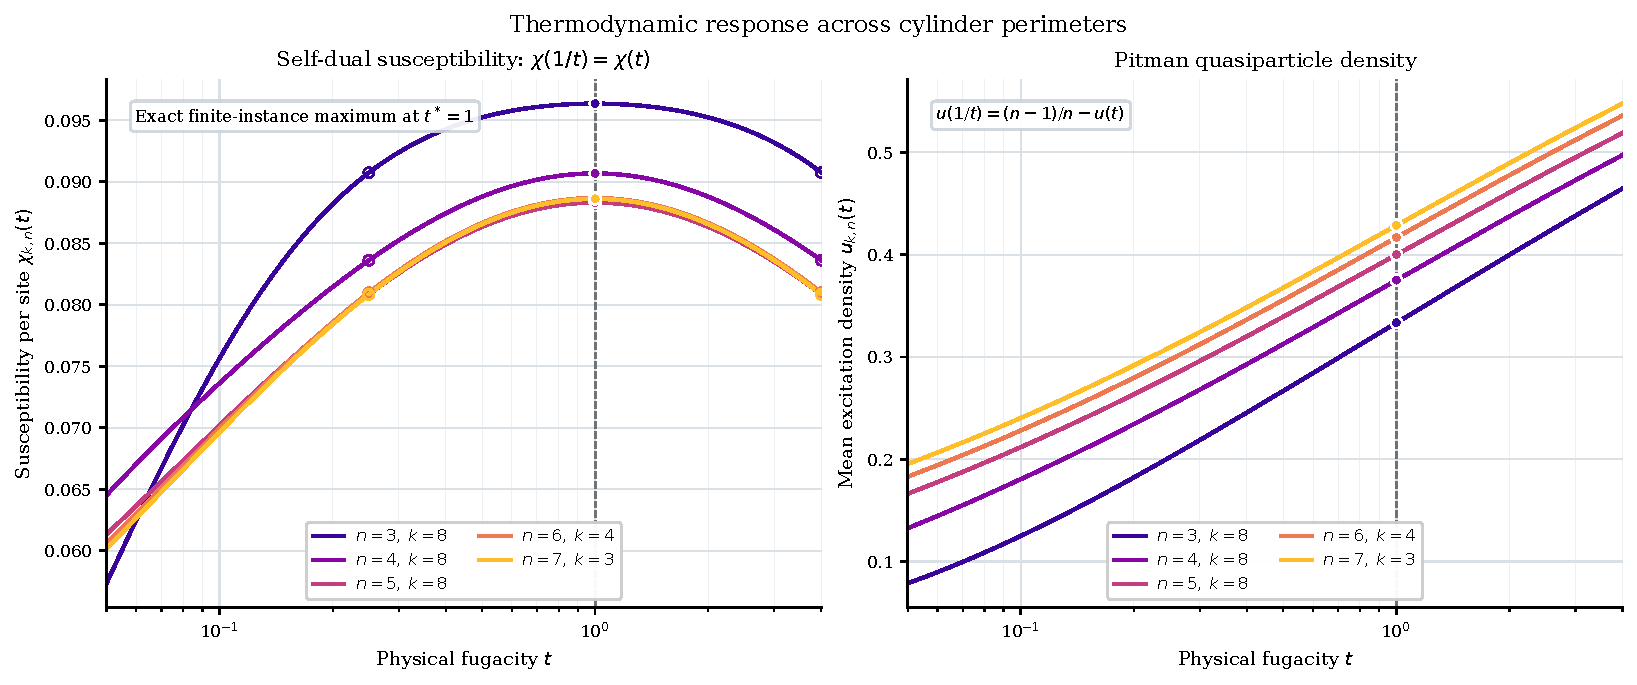
\includegraphics[width=0.97\linewidth]{fig_susceptibility_duality.pdf}
  \caption{Densidad de excitaciones de Pitman y susceptibilidad para la mayor longitud disponible en cada perímetro: $k=8$ para $n=3,4,5$, $k=4$ para $n=6$ y $k=3$ para $n=7$. Las curvas se evalúan a partir de las raíces de 50 dígitos. La relación recíproca exacta se muestra en $0.25\le t\le4$ y los marcadores centrales identifican el máximo global certificado $t^*=1$.}
  \label{fig:es-duality}
\end{figure}

\section{Brechas de Lee--Yang a perímetro finito y densidad BKW}

Sea $r_{\max}(k,n)$ el cero negativo más cercano a cero y $d_0(k,n)=|r_{\max}(k,n)|$. Para la familia $n=3$, el borde exacto de \eqref{eq:es-i3} implica
\[
  d_0(k,3)>7-4\sqrt3\quad(k\ge2).
\]
Para la recurrencia de orden tres de $n=4$ estudiada en el análisis fuente, el borde BKW viene determinado por
\[
  q_4(t)=t^4+76t^3-282t^2+76t+1,
  \quad z_0=-38-24\sqrt3,
  \quad \beta_+^{(4)}=\frac{z_0+\sqrt{z_0^2-4}}2,
\]
y las raíces finitas reportadas satisfacen $d_0(k,4)>|\beta_+^{(4)}|$. Numéricamente, los dos bordes inferiores son $7-4\sqrt3\simeq0.07179677$ y $|\beta_+^{(4)}|\simeq0.01256966$. La Fig.~\ref{fig:es-gap} muestra todos los valores disponibles de $d_0(k,n)$. Sus medias por perímetro descienden de $0.08749$ para $n=3$ a $0.0005469$ para $n=7$. Una regresión exponencial descriptiva de esas cinco medias es $\bar d_0(n)\simeq3.013e^{-1.256n}$, con $R^2=0.991$; como los rangos de $k$ disponibles difieren por perímetro, el ajuste no es una ley asintótica. Las razones de contracción a $k$ emparejado también varían: de $0.1994$ entre $n=3,4$ a $0.3094$ entre $n=6,7$.

\begin{figure}[htbp]
  \centering
  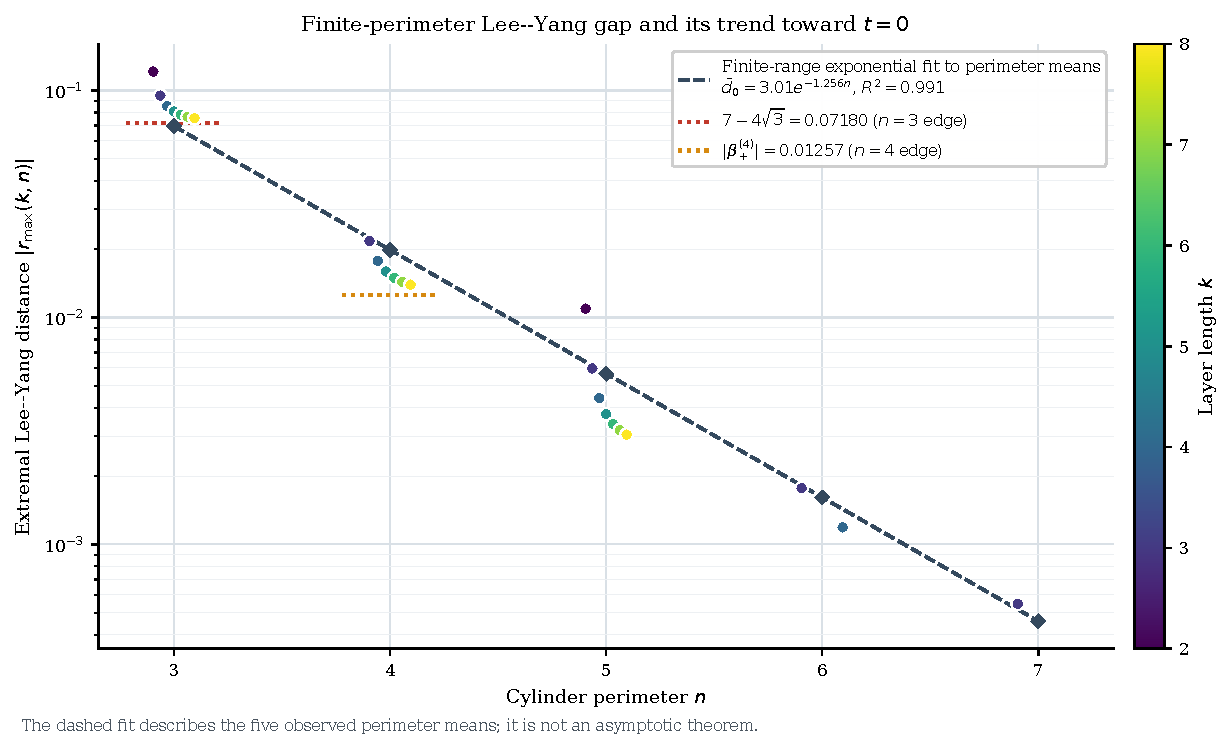
\includegraphics[width=0.94\linewidth]{fig_lee_yang_gap.pdf}
  \caption{Brecha de Lee--Yang $d_0=|r_{\max}(k,n)|$ en escala semilogarítmica para las 23 instancias, coloreadas por longitud $k$. Los segmentos horizontales muestran los bordes límite exactos de $n=3,4$. La línea discontinua ajusta únicamente las cinco medias de perímetro observadas.}
  \label{fig:es-gap}
\end{figure}

La Tabla~\ref{tab:es-instances} resume las 23 instancias finitas de ceros de Lee--Yang y termodinámica. Las raíces extremales están redondeadas a 12 cifras significativas; el archivo JSON contiene las listas completas refinadas a 50 cifras desde intervalos racionales exactos de Sturm. Aquí $D=k(n-1)$ es el grado del polinomio, y el mismo archivo incluye las mallas termodinámicas de 121 puntos.

\begin{landscape}
\tiny
\setlength{\tabcolsep}{2.3pt}
\renewcommand{\arraystretch}{1.22}
\begin{longtable}{@{}cc>{\raggedleft\arraybackslash}p{3.2cm}>{\raggedleft\arraybackslash}p{3.2cm}>{\raggedleft\arraybackslash}p{2.6cm}>{\raggedleft\arraybackslash}p{2.4cm}>{\centering\arraybackslash}p{1.0cm}>{\raggedleft\arraybackslash}p{2.6cm}@{}}
\caption{Datos finitos de ceros de Lee--Yang y termodin\'amica. Las ra\'ices extremales se redondean a 12 cifras significativas; las listas completas de 50 d\'igitos est\'an en el archivo JSON.}\label{tab:es-instances}\\
\toprule
\multicolumn{1}{c}{$k$} & \multicolumn{1}{c}{$n$} & \tableheading{3.2cm}{$r_{\min}$} & \tableheading{3.2cm}{$r_{\max}$} & \tableheading{2.6cm}{$d_0$} & \tableheading{2.4cm}{\shortstack{$\log_{10}$\\$(r_{\min}/r_{\max})$}} & \tableheading{1.0cm}{$t^*$} & \tableheading{2.6cm}{$\chi_{\max}$} \\
\midrule
\endfirsthead
\toprule
\multicolumn{1}{c}{$k$} & \multicolumn{1}{c}{$n$} & \tableheading{3.2cm}{$r_{\min}$} & \tableheading{3.2cm}{$r_{\max}$} & \tableheading{2.6cm}{$d_0$} & \tableheading{2.4cm}{\shortstack{$\log_{10}$\\$(r_{\min}/r_{\max})$}} & \tableheading{1.0cm}{$t^*$} & \tableheading{2.6cm}{$\chi_{\max}$} \\
\midrule
\endhead

2 & 3 & \tablevalue{-8.25108514330E+0} & \tablevalue{-1.21196179973E-1} & \tablevalue{1.21196179973E-1} & \tablevalue{1.83302213728E+0} & 1 & \tablevalue{1.04166666667E-1} \\
3 & 3 & \tablevalue{-1.05369769780E+1} & \tablevalue{-9.49038801251E-2} & \tablevalue{9.49038801251E-2} & \tablevalue{2.04543206234E+0} & 1 & \tablevalue{1.00694444444E-1} \\
4 & 3 & \tablevalue{-1.17161952468E+1} & \tablevalue{-8.53519405350E-2} & \tablevalue{8.53519405350E-2} & \tablevalue{2.13757320091E+0} & 1 & \tablevalue{9.89583333333E-2} \\
5 & 3 & \tablevalue{-1.23832885628E+1} & \tablevalue{-8.07539931681E-2} & \tablevalue{8.07539931681E-2} & \tablevalue{2.18567198646E+0} & 1 & \tablevalue{9.79166666667E-2} \\
6 & 3 & \tablevalue{-1.27923143686E+1} & \tablevalue{-7.81719375547E-2} & \tablevalue{7.81719375547E-2} & \tablevalue{2.21389824714E+0} & 1 & \tablevalue{9.72222222222E-2} \\
7 & 3 & \tablevalue{-1.30596050884E+1} & \tablevalue{-7.65719938110E-2} & \tablevalue{7.65719938110E-2} & \tablevalue{2.23186008886E+0} & 1 & \tablevalue{9.67261904762E-2} \\
8 & 3 & \tablevalue{-1.32432737360E+1} & \tablevalue{-7.55100302187E-2} & \tablevalue{7.55100302187E-2} & \tablevalue{2.24399071186E+0} & 1 & \tablevalue{9.63541666667E-2} \\
3 & 4 & \tablevalue{-4.60735733978E+1} & \tablevalue{-2.17044159212E-2} & \tablevalue{2.17044159212E-2} & \tablevalue{3.32690379359E+0} & 1 & \tablevalue{9.44865319865E-2} \\
4 & 4 & \tablevalue{-5.63395936570E+1} & \tablevalue{-1.77495067871E-2} & \tablevalue{1.77495067871E-2} & \tablevalue{3.50162742072E+0} & 1 & \tablevalue{9.29646880416E-2} \\
5 & 4 & \tablevalue{-6.27849422412E+1} & \tablevalue{-1.59273858397E-2} & \tablevalue{1.59273858397E-2} & \tablevalue{3.59571099812E+0} & 1 & \tablevalue{9.20495093666E-2} \\
6 & 4 & \tablevalue{-6.69691426589E+1} & \tablevalue{-1.49322502917E-2} & \tablevalue{1.49322502917E-2} & \tablevalue{3.65174947824E+0} & 1 & \tablevalue{9.14393185722E-2} \\
7 & 4 & \tablevalue{-6.98021797163E+1} & \tablevalue{-1.43262001855E-2} & \tablevalue{1.43262001855E-2} & \tablevalue{3.68773796914E+0} & 1 & \tablevalue{9.10034656703E-2} \\
8 & 4 & \tablevalue{-7.17946591975E+1} & \tablevalue{-1.39286126737E-2} & \tablevalue{1.39286126737E-2} & \tablevalue{3.71218427658E+0} & 1 & \tablevalue{9.06765759202E-2} \\
2 & 5 & \tablevalue{-9.14538399123E+1} & \tablevalue{-1.09344779941E-2} & \tablevalue{1.09344779941E-2} & \tablevalue{3.92240389021E+0} & 1 & \tablevalue{9.39516129032E-2} \\
3 & 5 & \tablevalue{-1.67913614690E+2} & \tablevalue{-5.95544323100E-3} & \tablevalue{5.95544323100E-3} & \tablevalue{4.45017182164E+0} & 1 & \tablevalue{9.15079365079E-2} \\
4 & 5 & \tablevalue{-2.26640334512E+2} & \tablevalue{-4.41227728574E-3} & \tablevalue{4.41227728574E-3} & \tablevalue{4.71067440503E+0} & 1 & \tablevalue{9.02341684294E-2} \\
5 & 5 & \tablevalue{-2.67051558472E+2} & \tablevalue{-3.74459525988E-3} & \tablevalue{3.74459525988E-3} & \tablevalue{4.85319023358E+0} & 1 & \tablevalue{8.94629147244E-2} \\
6 & 5 & \tablevalue{-2.94881532813E+2} & \tablevalue{-3.39119235600E-3} & \tablevalue{3.39119235600E-3} & \tablevalue{4.93929515074E+0} & 1 & \tablevalue{8.89480053470E-2} \\
7 & 5 & \tablevalue{-3.14418274510E+2} & \tablevalue{-3.18047671230E-3} & \tablevalue{3.18047671230E-3} & \tablevalue{4.99501556003E+0} & 1 & \tablevalue{8.85801388578E-2} \\
8 & 5 & \tablevalue{-3.28493654574E+2} & \tablevalue{-3.04419883329E-3} & \tablevalue{3.04419883329E-3} & \tablevalue{5.03305396965E+0} & 1 & \tablevalue{8.83042318189E-2} \\
3 & 6 & \tablevalue{-5.65745263491E+2} & \tablevalue{-1.76757997730E-3} & \tablevalue{1.76757997730E-3} & \tablevalue{5.50524185332E+0} & 1 & \tablevalue{8.97561710003E-2} \\
4 & 6 & \tablevalue{-8.41193092421E+2} & \tablevalue{-1.18878769810E-3} & \tablevalue{1.18878769810E-3} & \tablevalue{5.84979139551E+0} & 1 & \tablevalue{8.86748135954E-2} \\
3 & 7 & \tablevalue{-1.82862313954E+3} & \tablevalue{-5.46859535121E-4} & \tablevalue{5.46859535121E-4} & \tablevalue{6.52424842213E+0} & 1 & \tablevalue{8.86073318216E-2} \\
\endfoot
\end{longtable}
\end{landscape}

\subsection{Densidad de fase BKW y comparación finita}

Para $n=3$, los autovalores dominantes de \eqref{eq:es-n3-recurrence} forman un par conjugado en el intervalo negativo $I_3$. Si $\Psi_3(t)$ es la fase del autovalor del semiplano superior, la densidad normalizada límite es
\begin{equation}
  \rho_3(t)=\frac{1}{3\pi}\left|\frac{d\Psi_3}{dt}\right|.
  \label{eq:es-bkw-density}
\end{equation}
Para $n=4$ usamos el cúbico característico
\[
  \lambda^3-P_4(t)\lambda^2-Q_4(t)\lambda-R_4(t),
\]
con
\[
  P_4=t^3+23t^2+23t+1,\quad
  Q_4=7t^5-28t^4-22t^3-28t^2+7t,\quad
  R_4=t(t-1)^6(t+1).
\]
En el intervalo BKW $I_4=(\beta_-^{(4)},\beta_+^{(4)})$, $\Psi_4$ es el argumento de la raíz característica con parte imaginaria positiva y $\rho_4(t)=|\Psi_4'(t)|/(4\pi)$. La expresión para $n=4$ es condicional: la recurrencia de orden tres se verifica para un rango inicial finito en el trabajo fuente, mientras que su validez para todo $k$ es una hipótesis explícita de ese análisis BKW. Comparamos la fase con $H_{8,4}$ sin presentarla como teorema incondicional para toda la sucesión de Ehrhart.

La distribución acumulada empírica es $N_{8,n}(t)/(8n)$, donde $N_{8,n}(t)$ cuenta las raíces hasta $t$ en el intervalo negativo correspondiente. Para $n=3$, las masas totales BKW y empírica coinciden en $2/3$. Para $n=4$, la masa BKW integrada en la malla es $0.69212061$, frente a la masa empírica finita $0.75$ de $H_{8,4}$; conservamos esta diferencia finita en vez de renormalizar las curvas. La comparación se muestra en la Fig.~\ref{fig:es-bkw}.

\begin{figure}[htbp]
  \centering
  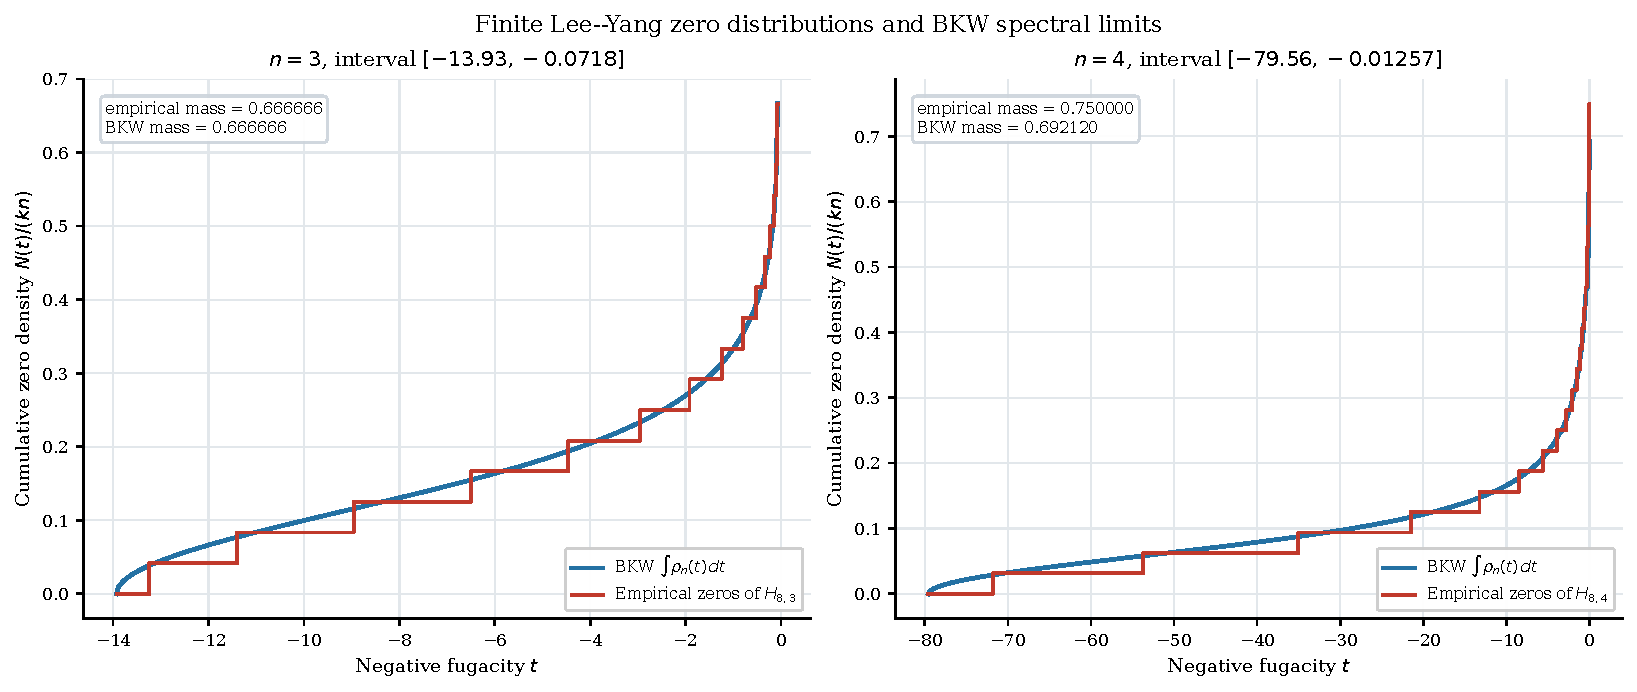
\includegraphics[width=0.97\linewidth]{fig_bkw_density.pdf}
  \caption{Distribuciones acumuladas empíricas de ceros de $H_{8,3}$ y $H_{8,4}$ frente a las integrales de sus densidades de fase BKW. La curva límite para $n=4$ usa la hipótesis condicional de recurrencia de orden tres y tiene una masa total menor que la muestra finita.}
  \label{fig:es-bkw}
\end{figure}

\section{Conclusión y reproducibilidad}

La correspondencia entre politopos de orden y P-particiones da una interpretación estadístico-mecánica exacta de los numeradores de Ehrhart cilíndricos. Para $n=3$, una transferencia exacta de dos modos demuestra la analiticidad de la energía libre a fugacidad positiva. En las 23 instancias finitas, las raíces recíprocas dan la factorización de Pitman, la autodualidad exacta y un certificado de coeficientes que localiza el máximo único de susceptibilidad en $t=1$. La distancia extremal de Lee--Yang decrece fuertemente en los perímetros observados; el ajuste exponencial resume los datos finitos y no prueba una ley asintótica uniforme. La comparación BKW de $n=4$ sigue condicionada a la hipótesis de recurrencia indicada.

El código fuente y los datos numéricos están en \texttt{LEE\_YANG\_PHYSICS/}. Las figuras se reproducen con \texttt{python generar\_graficas\_lee\_yang.py}; compile este manuscrito dos veces con \texttt{pdflatex}. El programa \texttt{analyze\_lee\_yang\_physics.py} vuelve a generar los datos JSON de polinomios, raíces y termodinámica.

\begin{thebibliography}{9}
\bibitem{LeeYang1952}
T. D. Lee y C. N. Yang,
Statistical theory of equations of state and phase transitions. II. Lattice gas and Ising model,
\emph{Physical Review} \textbf{87} (1952), 410--419.
\href{https://doi.org/10.1103/PhysRev.87.410}{doi:10.1103/PhysRev.87.410}.

\bibitem{Stanley1986}
R. P. Stanley,
Two poset polytopes,
\emph{Discrete \& Computational Geometry} \textbf{1} (1986), 9--23.
\href{https://doi.org/10.1007/BF02187680}{doi:10.1007/BF02187680}.

\bibitem{BKW1975}
S. Beraha, J. Kahane y N. Weiss,
Limits of zeros of recursively defined polynomials,
\emph{Proceedings of the National Academy of Sciences} \textbf{72} (1975), 4209--4211.
\href{https://doi.org/10.1073/pnas.72.11.4209}{doi:10.1073/pnas.72.11.4209}.

\bibitem{BeckRobins}
M. Beck y S. Robins,
\emph{Computing the Continuous Discretely: Integer-Point Enumeration in Polyhedra},
2nd ed., Springer, 2015.
\end{thebibliography}

\end{document}
